\documentclass[ignorenonframetext, professionalfonts, hyperref={pdftex, unicode}]{beamer}

\usetheme{Copenhagen}
\usecolortheme{wolverine}

%Packages to be included
%\usepackage{graphicx}

\usepackage[russian]{babel}
\usepackage[utf8]{inputenc}
\usepackage[T1]{fontenc}

%%\usepackage[orientation=landscape, size=custom, width=16, height=9.75, scale=0.5]{beamerposter}

\usepackage{textcomp}

\usepackage{beamerthemesplit}

\usepackage{ulem}

\usepackage{verbatim}

\usepackage{ucs}


\usepackage{listings}
\lstloadlanguages{bash}

\lstset{escapechar=`,
	extendedchars=false,
	language=sh,
	frame=single,
	tabsize=2, 
	columns=fullflexible, 
%	basicstyle=\scriptsize,
	keywordstyle=\color{blue}, 
	commentstyle=\itshape\color{brown},
%	identifierstyle=\ttfamily, 
	stringstyle=\mdseries\color{green}, 
	showstringspaces=false, 
	numbers=left, 
	numberstyle=\tiny, 
	breaklines=true, 
	inputencoding=utf8,
	keepspaces=true,
	morekeywords={u\_short, u\_char, u\_long, in\_addr}
	}

\definecolor{darkgreen}{cmyk}{0.7, 0, 1, 0.5}

\lstdefinelanguage{diff}
{
    morekeywords={+, -},
    sensitive=false,
    morecomment=[l]{//},
    morecomment=[s]{/*}{*/},
    morecomment=[l][\color{darkgreen}]{+},
    morecomment=[l][\color{red}]{-},
    morestring=[b]",
}

\author[Epam]{{\bf Epam}\\Low Level Programming Department}

%\institution[EPAM]{EPAM}
%\logo{\includegraphics[width=1cm]{logo.png}}

\title{Введение в GNU/Linux\\Командная строка}

\begin{document}
\begin{frame}
 \frametitle{}
 \titlepage
\end{frame}
\section{Полезные инструменты bash}
\mode<all>{\begin{frame}{Важные аббревиатуры внутри командной строки}
  \begin{itemize}
    \item Для директорий
      \begin{itemize}
        \item {\tt $\sim$} Домашняя директория
        \item {\tt $\sim$<username>} Домашняя директория пользователя
        \item {\tt ..} Родительская директория
        \item {\tt .} Текущая директория
      \end{itemize}
      \pause  
    \item Wildcards
      \begin{itemize}
        \item {\tt *} Любой набор символов {\tt file*txt : file1.txt filefilefiletxt}
        \item {\tt $[$<список>$]$ } символ из заданного набора
        \item {\tt ?} любой один символ
      \end{itemize}

  \end{itemize}
\end{frame}       

\begin{frame}{Горячие клавиши}
  \begin{itemize}
    \item \textbf{Tab} -- дополнение текущей команды
      \pause
    \item История команд
      \begin{itemize}
        \item Клавиши курсора -- навигация по истории
        \item Ctrl-R -- поиск в истории по фрагменту
        \item Ctrl-O (после выполнения вставить следующую команду из истории)
        \item Команда {\tt history}
      \end{itemize}
    \item Навигация

  \end{itemize}
\end{frame}

\begin{frame}{Переменные окружения}
  \begin{itemize}
    \item {\tt HOME}
    \item {\tt PWD}
    \item {\tt LANG}
    \item {\tt LD\_LIBRARY\_PATH}
    \item {\tt SHELL}
    \item {\tt TERM}
    \item {\tt DISPLAY}
  \end{itemize}

  Контроль

  \begin{itemize}
    \item export {\tt export VAR=value}
    \item declare -x
    \item echo 
  \end{itemize}

  Переменные окружения наследуются при создании нового процесса
\end{frame}

%\begin{frame}{Настройки bash и кастомизация}
%  \begin{itemize}
%    \item Login shell
%      \begin{itemize}
%        \item {\tt /etc/profile}
%        \item {\tt $\sim$/.profile }
%      \end{itemize}
%    \item Обычная интерактивная shell
%      \begin{itemize}
%        \item {\tt /etc/bash.bashrc}
%        \item {\tt $\sim$/.bashrc}
%      \end{itemize}
%  \end{itemize}
%
%  Полезные команды
%  \begin{itemize}
%    \item {\tt alias}
%    \item {\tt export PATH=}
%    \item {\tt Определение функции}
%    \item {\tt shopts}
%  \end{itemize}
%
%\end{frame}


}

\section{Процессы}
\mode<all>{\begin{frame}{Процессы в UNIX}
  \begin{itemize}
    \item Создание процессов
      \begin{itemize}
        \item fork
        \item exec
      \end{itemize}
    \item Атрибуты процесса
      \begin{itemize}
        \item pid 
        \item файловые дескрипторы
        \item environment
        \item Рабочая директория (cwd)
        \item прочее в директории {\tt /proc/<pid>}
      \end{itemize}
  \end{itemize}
\end{frame}

\begin{frame}{Управление процессами}
  \begin{itemize}
    \item kill (killall)
    \item top
    \item pstree
    \item Команды управления процессами в bash: 
      \begin{itemize}
        \item {\tt jobs}, {\tt fg, \tt bg}
        \item Ctrl-C -- оборвать выполнение процесса (SIGINT)
        \item Ctrl-Z -- остановить выполнение команды (SIGTSTP)
        \item Ctrl-D -- завершить ввод
      \end{itemize}
  \end{itemize}
\end{frame}


\begin{frame}{Упражнения}
  \begin{block}{Посмотреть вывод pstree}
    {\tt pstree}
  \end{block}
  \pause
  \begin{block}{Ctrl-C, Ctrl-Z}
    В графическом режиме запустить из терминала emacs

    Ctrl-Z

    jobs -l

    bg +
  \end{block}
  \pause
  \begin{block}{fork bomb}

    {\tt ulimit -u 200} 

    {\tt bomb()\{ (bomb; bomb) \& \} }

    top

    killall bash

  \end{block}
\end{frame}


\begin{frame}{Unix way}
  \begin{enumerate}
    \item Пишите программы, которые делают одну вещь и делают её хорошо.
    \item Пишите программы, которые бы работали вместе.
    \item Пишите программы, которые бы поддерживали текстовые потоки, поскольку это универсальный интерфейс. 
  \end{enumerate}
\end{frame}

\begin{frame}{Unix way}
  \begin{enumerate}
    \item   Маленькое прекрасно.
    \item   Пусть каждая программа делает одну вещь, но хорошо.
    \item   Собирайте прототип как можно раньше.
    \item   Предпочитайте переносимость эффективности.
    \item   Храните данные в простых текстовых файлах.
    \item   Используйте программные рычаги для достижения цели.
    \item   Используйте сценарии командной строки для улучшения функционала и переносимости.
    \item   Избегайте <<связывающего>> (captive) пользовательского интерфейса.
    \item   Делайте каждую программу «фильтром».
  \end{enumerate}
\end{frame}

\begin{frame}{Конвееры}
%  \textbf{Цель} -- максимальная модульность: большое количество простых приложений, взаимодействующих друг с другом для решения задач
  \only<1>{
  \begin{center}
    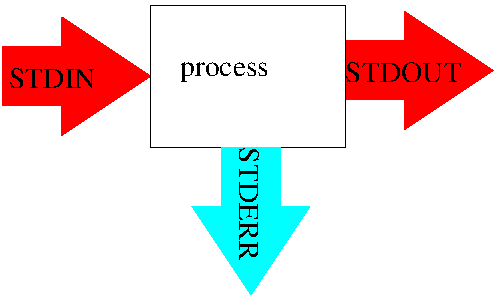
\includegraphics[width=1.2in]{../../slides/cmdline/process}
  \end{center}
  }
  \only<2>{
    \begin{center}
      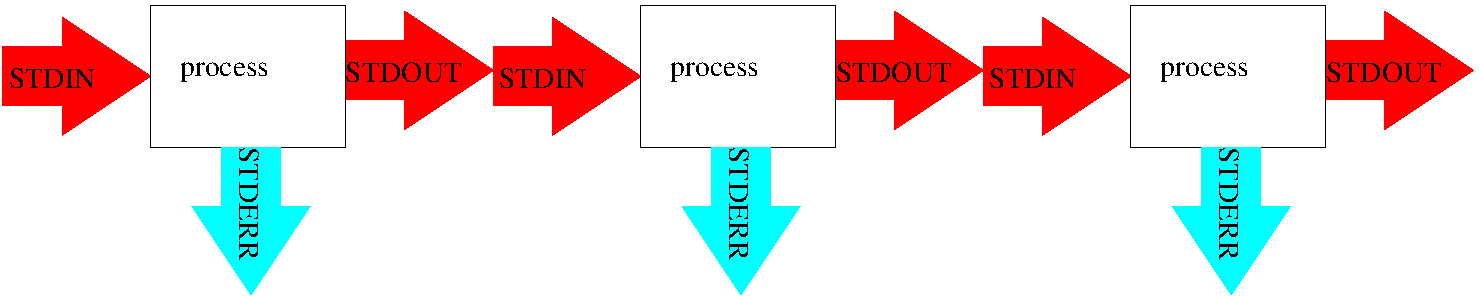
\includegraphics[width=3.6in]{../../slides/cmdline/processes}
    \end{center}
  }
  \begin{itemize}
    \item <1-> Каждое приложение открывает 3 стандартных файловых дескриптора stdin (fd 0), stdout(fd 1), stderr (fd 2)
    \item <2-> Приложения могут работать как фильтр из STDIN в STDOUT, можно объединять несколько приложений в конвейер
    \item <2-> Синтаксис {\tt <app1> | <app2>}
  \end{itemize}
\end{frame}
}

\section{Перенаправление ввода-вывода}
\mode<all>{

\begin{frame}{Конвееры}
%  \textbf{Цель} -- максимальная модульность: большое количество простых приложений, взаимодействующих друг с другом для решения задач
  \only<1>{
  \begin{center}
    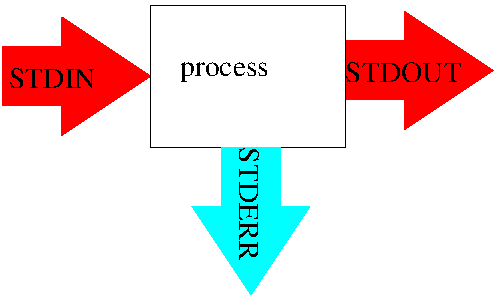
\includegraphics[width=1.2in]{../../slides/cmdline/process}
  \end{center}
  }
  \only<2>{
    \begin{center}
      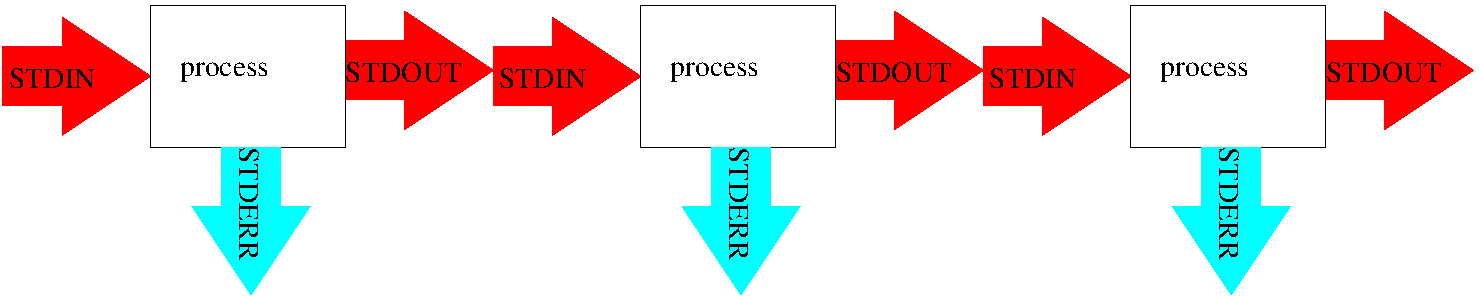
\includegraphics[width=3.6in]{../../slides/cmdline/processes}
    \end{center}
  }
  \begin{itemize}
    \item <1-> Каждое приложение открывает 3 стандартных файловых дескриптора stdin (fd 0), stdout(fd 1), stderr (fd 2)
    \item <2-> Приложения могут работать как фильтр из STDIN в STDOUT, можно объединять несколько приложений в конвейер
    \item <2-> Синтаксис {\tt <app1> | <app2>}
  \end{itemize}
\end{frame}
}
\mode<all>{\begin{frame}{Перенаправления в файл}

\begin{itemize}
  \item Перенаправление stdout 
    \begin{itemize}
      \item С созданием нового файла

        {\tt command > file}\\
		Например {\tt cat file1 file2 > file3}
      \item С дополнением существующего

		  {\tt command >\phantom{}>  file}
    \end{itemize}
    \pause
  \item Перенаправления stdin

    {\tt command < file}
    \pause
  \item Перенаправления stderr

    {\tt command1 2>\&1 | command2}

   {\tt command 1>file 2>\&1}

   {\tt command 2>file 1>\&2}
\end{itemize}

\end{frame}


}
\mode<all>{\begin{frame}[fragile]{Мультистрочный ввод (Here-документ)}

\begin{verbatim}
program <<LABEL
Тут
    много
	     строк
LABEL
\end{verbatim}

	\pause
	\begin{block}{Пример}
	Передадим несколько строк в COM-порт 1
\begin{lstlisting}[language=bash]
cat >/dev/ttyS0 <<E_O_F
ATZ
ATDT 8w0170123456
E_O_F
\end{lstlisting}
	\end{block}
\end{frame}
}

\section{Полезные команды}

\mode<all>{\begin{frame}{Дополнительный набор команд}
  \begin{itemize}
    \item {\tt cat} - Вывод файла в stdout, соединение нескольких файлов в stdout
    \item {\tt wc} - подсчет статистики символов в файле или в stdin 
    \item {\tt sort} - сортировка строк файла
    \item {\tt uniq} - объединение одинаковых строк в одну
    \item {\tt tr} - замена набора символов
    \item {\tt less} - программа-пейджер
    \item {\tt grep} - поиск строк, соответствующих регулярному выражению
    \item {\tt cut} - выделение полей из строк stdin
    \item {\tt awk} - небольшой язык программирования (также полезен для выделения полей)
  \end{itemize}
\end{frame}

\begin{frame}[fragile]{Некоторые примеры использования}
\begin{lstlisting}[language=bash]
cat /proc/1/environ | tr '\0' '\n' | less
ls  | wc -l # подсчет числа файлов
man uniq | tr  '[:space:]' '\n' | sort | uniq -c | sort -n | less # подсчет количества слов в тексте man uniq
history | wc -l # подсчет ранее введенных команд
cat /etc/udev/rules.d/* | wc -l
ls -s *.jpg | awk 'BEGIN{s=0};/^[ ]*[0-9]/{s+=\$1};END{print s}' 
\end{lstlisting}
  \pause
  \begin{block}{Упражнение}
    Посчитать статистику использования команд в history
  \end{block}
\end{frame}

\begin{frame}{Дополнительный набор команд для работы с текстом}
	\begin{itemize}
	  \item {\tt head} -- вывести первые строки
	  \item {\tt tail} -- вывести последние строки
		\begin{itemize}
			\item {\tt -f} -- отслеживать добавление данных в файл 
		\end{itemize}
	  \item {\tt tee} -- копировать стандартный вывод в файл
	  \item {\tt grep} -- печать текста, соответствующего шаблону
		\begin{itemize}
			\item {\tt -i}	
			\item {\tt -v}
			\item {\tt -o}
		\end{itemize}
	\end{itemize}
\end{frame}

}

\end{document}
